\chapter{Implementación}\label{cap:implementacion}
\Juanmi[]{Punto a revisar}

En este capítulo se describe la implementación del proyecto, así como detalles técnicos y decisiones tomadas durante el desarrollo. Se divide en varios sprints, cada uno con sus propias tareas y objetivos.

\section{Sprint 0}

En este sprint no se comienza el desarrollo del proyecto, sino que, como se menciona en la seccion \ref{cap:especificación} y \ref{cap:planificacion}, se realiza una investigación sobre las tecnologías a utilizar, y se detallan los requerimientos del sistema, y la arquitectura a implementar.
\newline\newline
Al usar Java como lenguaje de programación y Spring Boot como framework de desarrollo, se sigue un patrón similar para el desarrollo de los servicios, ya que todos comparten componentes y directorios similares.

\subsection{Estructura general de los servicios}

El código fuente de los servicios se organiza en paquetes, siguiendo una estructura común para todos los servicios. Esta estructura incluye:

\begin{itemize}
    \item \textbf{config}: Contiene la configuración del servicio, como la configuración de seguridad, bases de datos, etc.
    \item \textbf{controller}: Contiene los controladores REST que manejan las peticiones HTTP.
    \item \textbf{dto}: Contiene los objetos de transferencia de datos (DTO) utilizados para la comunicación entre el cliente y el servidor.
    \item \textbf{model}: Contiene las entidades del dominio del servicio.
    \item \textbf{repository}: Contiene las interfaces de repositorio que extienden de JPA para la persistencia de datos.
    \item \textbf{service}: Contiene la lógica de negocio del servicio.
    \item \textbf{mapper}: Contiene los mapeadores para convertir entre entidades y DTOs.
    \item \textbf{Application.java}: Clase principal que arranca el servicio.
\end{itemize}

De esta forma, se consigue una estructura clara y coherente para el desarrollo de los servicios, facilitando la comprensión y el mantenimiento del código.

Además para la configuración de estos, se utiliza un archivo de propiedades (application.properties) que permite definir las propiedades específicas del servicio, como la conexión a la base de datos, el puerto en el que se ejecuta el servicio, etc.

\section{Sprint 1}

Este primer sprint se comienza con cierta incertidumbre al no haber tenido todavía la reunión con Alberto Guillén Perales, el director del CEPRUD, por lo que no se sabe a qué información se va a tener acceso, y por tanto cómo se van a implementar ciertas funcionalidades.
\newline\newline
Sin embargo, ya que el proceso para poder hacer uso del sistema de autenticación de la UGR parece ser largo y requiere de una serie de permisos y pasos previos \cite{autenticacion_ugr}, se decide en este punto comenzar a implementar en el backend todas las funcionalidades relacionadas con la gestión de usuarios, y autenticación basadas en las credenciales de la UGR.
\newline\newline
Para conseguir esto se implementan los servicios ``User Service'', ``Auth Service'', ``Mail Service'' y el ``API Gateway''.

\subsection{User Service}

Este servicio se plantea como el encargado de gestionar los usuarios del sistema, permitiendo registrar, consultar, actualizar y eliminar usuarios. Además, se encarga de la gestión de roles y permisos, así como de la codificación de contraseñas.
\newline 
Las contraseñas se almacenan de forma segura mediante codificación (por ejemplo, \texttt{BCrypt}), y no en texto plano.
\newline\newline
Los usuarios pueden poseer los roles de \texttt{ROLE\_INACTIVE}, \texttt{ROLE\_STUDENT}, \texttt{ROLE\_TEACHER}, o \texttt{ROLE\_ADMIN}, y estos nos permiten controlar el acceso a diferentes funcionalidades del sistema.
\newline\newline
Aunque este servicio no es el encargado de la autenticación, srve de soporte para el servicio de autenticación, proporcionando la información de los usuarios y sus roles.

\subsubsection{Integración con otros microservicios}

\begin{itemize}
  \item Es consultado por otros servicios para validar identidad o permisos de los usuarios.
  \item Envía mensajes mediante RabbitMQ para notificar el registro de usuarios y/o cambios en sus credenciales.
\end{itemize}

\subsubsection{Diagrama de clases}
Este es el primer servicio implementado, y se sigue una estructura similar en los demás servicios para mantener la coherencia en el proyecto. La arquitectura de los servicios en la \textbf{Arquitectura limpia o hexagonal}, que se basa en la separación de responsabilidades y la independencia de las capas, se refleja en el diagrama de clases del servicio User Service, que se muestra en la figura \ref{fig:user-service-class-diagram}.
\begin{figure}[H]
    \centering
    \makebox[\textwidth][c]{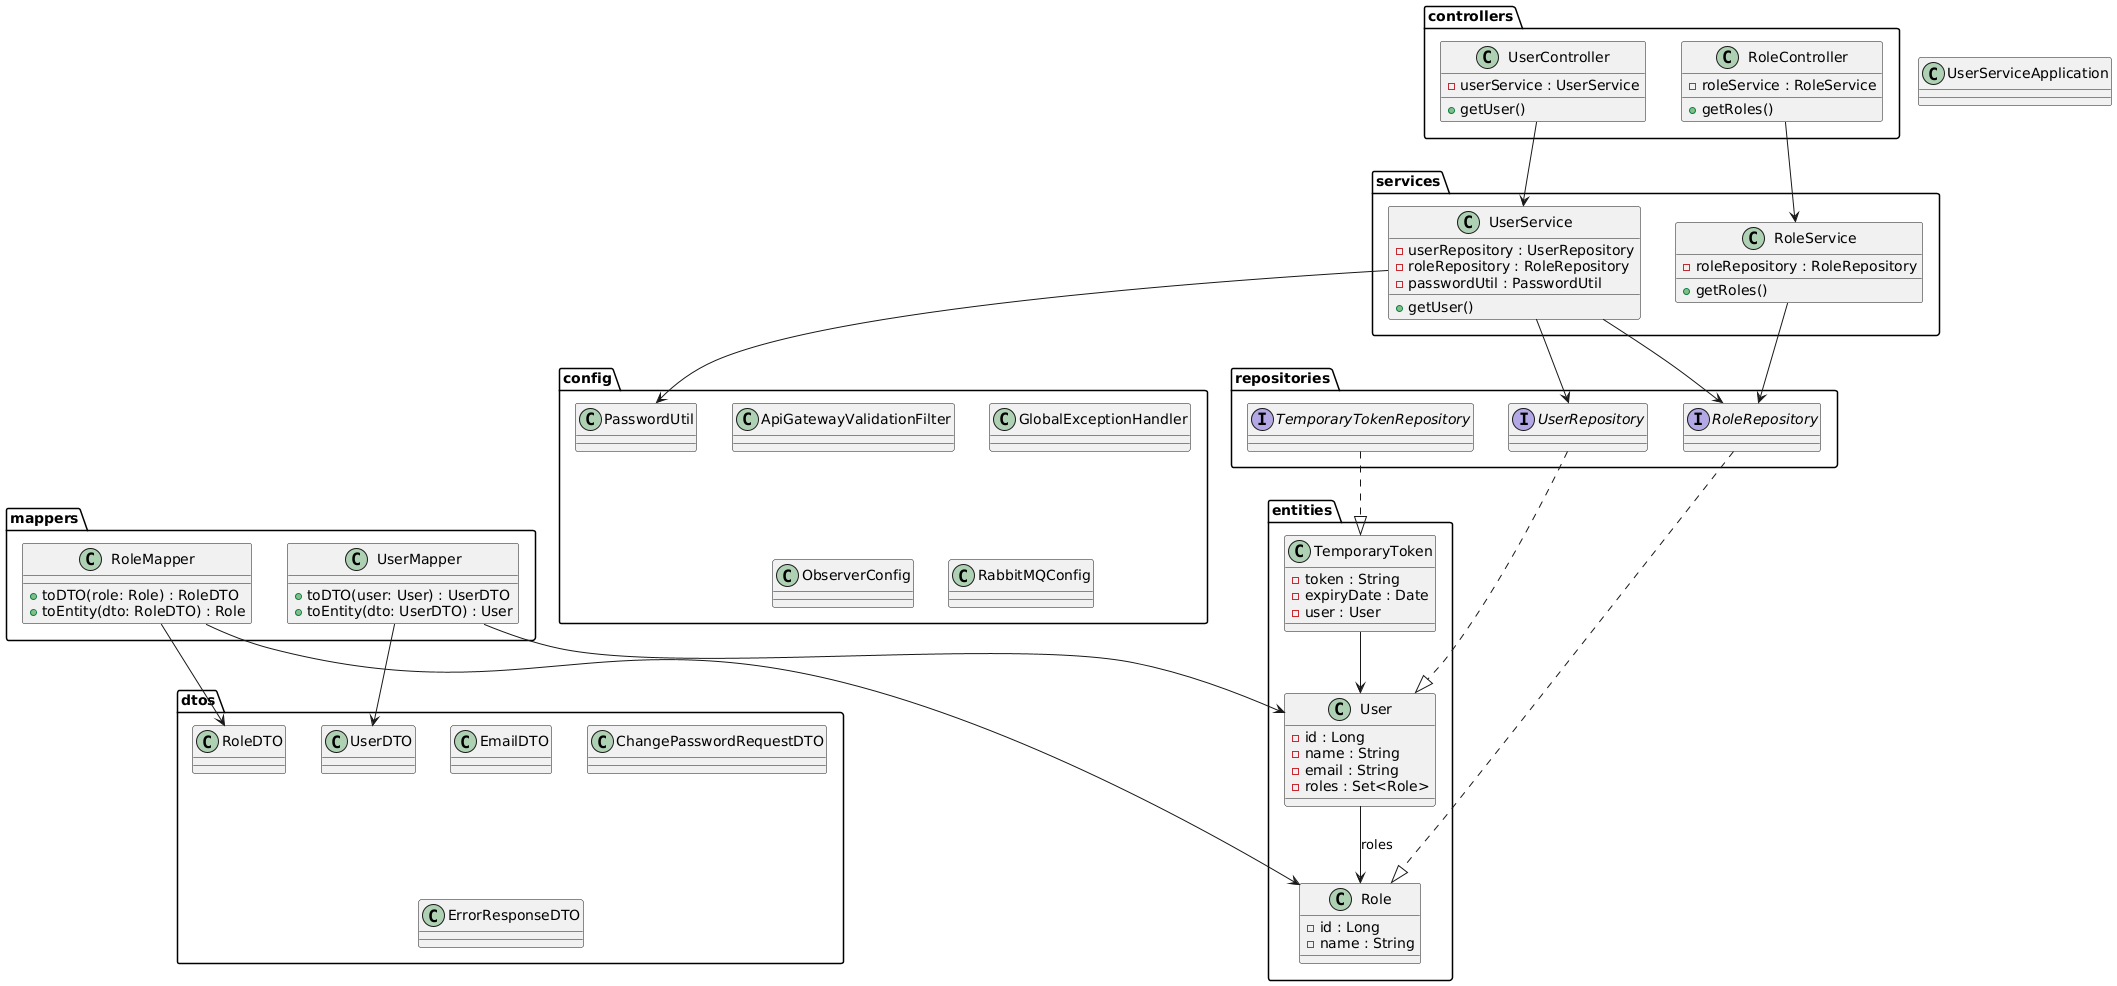
\includegraphics[width=1.2\textwidth]{figures/07_uml_user.png}}
    \caption{Diagrama de clases del servicio User Service realizado con PlantUML}
    \label{fig:user-service-class-diagram}
\end{figure}

Este diagrama representa las principales clases del servicio, incluyendo los controladores, servicios, repositorios y entidades. Cada clase tiene una responsabilidad clara y se comunica con otras clases a través de interfaces, lo que permite una fácil extensibilidad y mantenimiento del código.

\subsubsection{Interacción entre componentes}

\subsubsection*{1. Controladores (\texttt{controllers})}

\begin{itemize}
  \item \textbf{UserController} y \textbf{RoleController}: Son clases que exponen endpoints HTTP. Actúan como punto de entrada de las solicitudes del cliente.
  \item \textbf{Interacción}: Invocan métodos en los servicios correspondientes (\texttt{UserService}, \texttt{RoleService}) para obtener datos o ejecutar lógica de negocio.
\end{itemize}

\subsubsection*{2. Servicios (\texttt{services})}

\begin{itemize}
  \item \textbf{UserService}: Contiene la lógica de negocio relacionada con usuarios.
    \begin{itemize}
      \item Depende de \texttt{UserRepository} y \texttt{RoleRepository} para acceder a la base de datos.
      \item Usa \texttt{PasswordUtil} para tareas relacionadas con contraseñas (encriptación, validación, etc).
    \end{itemize}
  \item \textbf{RoleService}: Contiene lógica de negocio asociada a roles.
    \begin{itemize}
      \item Se comunica con \texttt{RoleRepository}.
    \end{itemize}
\end{itemize}

\subsubsection*{3. Repositorios (\texttt{repositories})}

\begin{itemize}
  \item \textbf{UserRepository}, \textbf{RoleRepository}, \textbf{TemporaryTokenRepository}: Son interfaces que definen operaciones CRUD (Create, Read, Update, Delete) sobre las entidades.
  \item \textbf{Interacción}: Son utilizados por los servicios para obtener o almacenar datos en la base de datos.
\end{itemize}

\subsubsection*{4. Entidades (\texttt{entities})}

\begin{itemize}
  \item \textbf{User}: Representa un usuario del sistema. Tiene atributos como \texttt{id}, \texttt{name}, \texttt{email}, y una colección de \texttt{roles}.
  \item \textbf{Role}: Representa un rol o permiso dentro del sistema. Se relaciona con los usuarios.
  \item \textbf{TemporaryToken}: Usado para funcionalidades temporales como recuperación de contraseña. Contiene un \texttt{token}, una fecha de expiración y referencia al \texttt{User}.
  \item \textbf{Interacción}: Estas entidades son gestionadas por los repositorios y utilizadas en la lógica de negocio de los servicios.
\end{itemize}

\subsubsection*{5. Mapeadores (\texttt{mappers})}

\begin{itemize}
  \item \textbf{UserMapper} y \textbf{RoleMapper}: Se encargan de convertir entidades (\texttt{User}, \texttt{Role}) a sus correspondientes objetos de transferencia de datos (\texttt{UserDTO}, \texttt{RoleDTO}) y viceversa.
  \item \textbf{Interacción}: Usados por los servicios para traducir datos entre capas internas y externas.
\end{itemize}

\subsubsection*{6. DTOs (\texttt{dtos})}

\begin{itemize}
  \item \textbf{UserDTO}, \textbf{RoleDTO}, \textbf{EmailDTO}, \textbf{ChangePasswordRequestDTO}, \textbf{ErrorResponseDTO}: Representan estructuras de datos que se usan para enviar y recibir información a través de la API.
  \item \textbf{Interacción}: Son utilizados por los controladores y servicios para comunicar información de forma segura y controlada, evitando exponer entidades directamente.
\end{itemize}

\subsubsection*{7. Configuración (\texttt{config})}

\begin{itemize}
  \item \textbf{PasswordUtil}: Clase de utilidad para el manejo de contraseñas.
  \item \textbf{ApiGatewayValidationFilter}: Filtro que valida solicitudes entrantes desde el API Gateway.
  \item \textbf{GlobalExceptionHandler}: Captura y maneja excepciones globalmente.
  \item \textbf{RabbitMQConfig}, \textbf{ObserverConfig}: Configuración para mensajería y observadores (por ejemplo, eventos asincrónicos).
  \item \textbf{Interacción}: Algunas de estas clases son inyectadas en servicios (\texttt{PasswordUtil}), otras se ejecutan automáticamente (\texttt{GlobalExceptionHandler}).
\end{itemize}

\subsubsection*{8. Flujo de Interacción General}

\begin{enumerate}
  \item El cliente realiza una solicitud a través del \texttt{UserController} o \texttt{RoleController}.
  \item El controlador llama al servicio correspondiente (\texttt{UserService} o \texttt{RoleService}).
  \item El servicio accede a los repositorios para obtener datos desde las entidades.
  \item Se usan los mapeadores para convertir entidades en DTOs.
  \item El DTO es devuelto al cliente a través del controlador.
\end{enumerate}

Aunque en cada servicio se implementan diferentes funcionalidades, la estructura y la interacción entre los componentes siguen un patrón similar, lo que facilita la comprensión del código.

\subsection{Mail Service}
El servicio de correo electrónico se encarga de enviar correos electrónicos a los usuarios del sistema. Este servicio es utilizado por otros servicios para enviar notificaciones, como la confirmación de registro, recuperación de contraseña, etc.

Su desarrollo combina tres tecnologías clave: \textbf{RabbitMQ}, \textbf{JavaMail} y \textbf{Thymeleaf}, permitiendo una integración fluida entre mensajería asíncrona y generación dinámica de contenido de correo.

El proceso comienza cuando otro componente del sistema necesita enviar un correo electrónico. En lugar de enviarlo directamente, publica un mensaje en una cola gestionada por \texttt{RabbitMQ}. Este servicio actúa como consumidor de esos mensajes mediante el uso de \texttt{listeners}, que reciben el contenido del mensaje en tiempo real. Esta estrategia permite desacoplar el proceso de envío de correo del resto de la lógica de negocio, mejorando la escalabilidad y la resiliencia del sistema ante posibles errores.

Una vez recibido el mensaje, el servicio extrae los datos necesarios, como la dirección de correo del destinatario, el asunto, y las variables que se inyectarán en el contenido. Para la composición del cuerpo del correo, se utiliza \texttt{Thymeleaf}, un motor de plantillas que permite construir correos HTML personalizados. Gracias a Thymeleaf, se pueden generar correos enriquecidos visualmente, dinámicos y adaptados al contexto de cada notificación, manteniendo una presentación clara y profesional.

Después de generar el contenido del correo, se utiliza la biblioteca \texttt{JavaMail} para su envío. JavaMail proporciona una API robusta y configurable que permite construir mensajes MIME, manejar los encabezados, adjuntos y establecer la conexión con el servidor SMTP. En este caso, se ha configurado el servicio para utilizar \textbf{Gmail como proveedor de correo electrónico}, lo cual requiere definir parámetros como el host SMTP de Gmail (\texttt{smtp.gmail.com}), el puerto correspondiente, y habilitar la autenticación y conexión segura mediante TLS. Esta configuración se especifica en los archivos de propiedades del servicio, lo que facilita su adaptación a distintos entornos de despliegue.

En conjunto, este microservicio representa una solución elegante y modular para el envío de correos en arquitecturas basadas en microservicios. Aprovecha la comunicación asincrónica de RabbitMQ, la potencia expresiva de las plantillas Thymeleaf, y la fiabilidad de JavaMail para lograr un sistema de notificaciones por correo eficaz, personalizable y mantenible.

\begin{figure}[H]
    \centering
    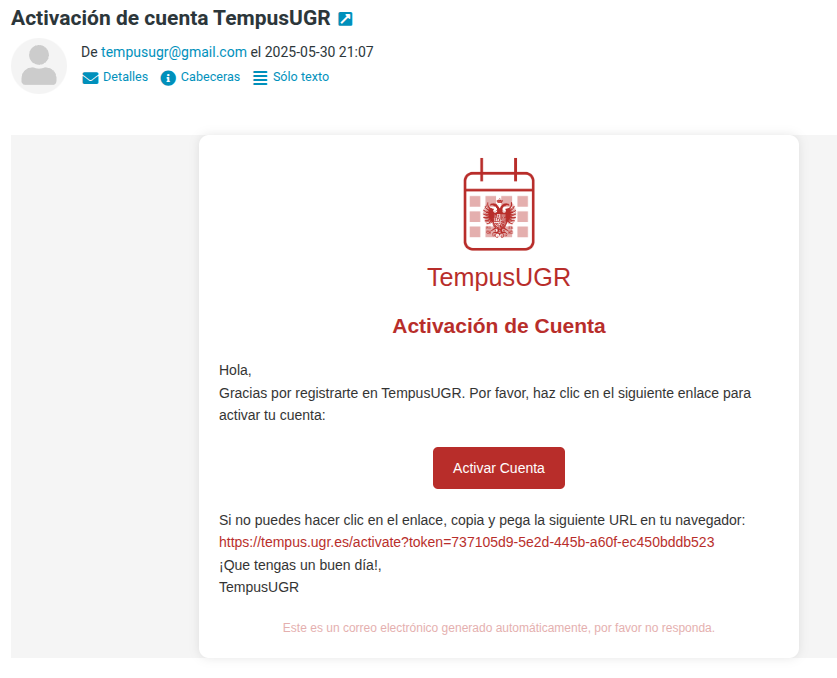
\includegraphics[width=0.8\textwidth]{figures/07_email.png}
    \caption{Correo de activación de cuenta}
    \label{fig:mail-service-class-diagram}
\end{figure}

\subsection{Auth Service}
El servicio de autenticación es el encargado de gestionar la autenticación de los usuarios del sistema. Este servicio se encarga de validar las credenciales de los usuarios y generar tokens JWT (JSON Web Tokens) para autenticar las solicitudes a otros servicios.
\newline\newline
Su lógica reside en la clase \texttt{AuthService}. 
La operación principal, \texttt{authenticate}, recibe las credenciales enviadas por el cliente y devuelve un par de tokens
\emph{JSON Web Token} (JWT): un \emph{access token} de corta duración y un \emph{refresh token} de duración más amplia. 

El proceso comienza verificando que la dirección de correo pertenezca a la Universidad de Granada; 
de lo contrario, se aborta la autenticación.  
Después, mediante un \texttt{WebClient} reactivo, el servicio consulta al microservicio de usuarios 
(\texttt{user-service}) para recuperar el \texttt{UserDTO} correspondiente.  
Si el usuario existe, está activo y la contraseña coincide con el \emph{hash} almacenado (comprobación
delegada a \texttt{PasswordUtil}), se generan ambos tokens.

\subsubsection*{Estructura del JWT}

Un JWT es una cadena en tres partes \emph{``header.payload.signature''}, codificadas en \texttt{Base64Url}.  
En este servicio se firma con el algoritmo simétrico \texttt{HS256}, usando la clave secreta
\lstinline|JWT_SECRET|:

\begin{verbatim}
Key key = Keys.hmacShaKeyFor(SECRET_KEY.getBytes(StandardCharsets.UTF_8));
String jwt = Jwts.builder()
        .setHeaderParam("typ", "JWT")
        .setSubject(id)              // Identificador del usuario
        .claim("role", role)         // Rol de la aplicación
        .setIssuedAt(new Date(now))
        .setExpiration(new Date(now + ttl))
        .signWith(key, SignatureAlgorithm.HS256)
        .compact();
\end{verbatim}

La cabecera (\texttt{header}) indica el tipo de token y el algoritmo de firma.  
El cuerpo (\texttt{payload}) almacena el identificador del usuario (\texttt{sub}), su rol y las marcas
temporal de emisión y caducidad (\texttt{iat}, \texttt{exp}).  
La firma garantiza la integridad: si cualquier byte del token cambia, la verificación falla.

\subsubsection*{Duración y refresco}

El \emph{access token} caduca en 24~horas (86,400,000~ms), su vida corta limita el riesgo ante robo.  
El \emph{refresh token} dura una semana y sólo sirve para
obtener nuevos \emph{access tokens}.  
La operación \texttt{refresh} valida la firma y la vigencia del \emph{refresh token};  
si supera la comprobación, crea un nuevo \emph{access token} manteniendo el \emph{refresh token} 
original mientras no haya expirado.  
El servidor no almacena sesiones, por lo que el mecanismo es \emph{stateless} y escalable: basta con
compartir la misma \lstinline|JWT_SECRET| entre las instancias.

\subsubsection*{Flujo de autenticación}

El diseño evita guardar estado en la base de datos y permite balancear las peticiones entre múltiples
réplicas sin afinidad de sesión.  

El flujo de autenticación y generación de tokens JWT se ilustra en la figura \ref{fig:auth-service-class-diagram}, donde se muestra cómo el servicio interactúa con el \texttt{user-service} para validar las credenciales y generar los tokens necesarios.

\begin{figure}[H]
    \centering
    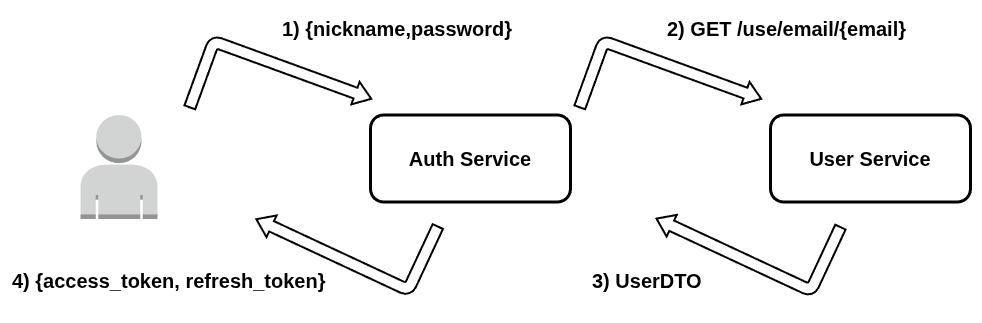
\includegraphics[width=0.8\textwidth]{figures/07_auth.png}
    \caption{Flujo de autenticación y generación de tokens JWT}
    \label{fig:auth-service-class-diagram}
\end{figure}

\subsection{API Gateway}
El \texttt{api-gateway} actúa como el punto de entrada centralizado para todas las peticiones del sistema basado en microservicios. Está construido utilizando \textbf{Spring Cloud Gateway}, una solución reactiva que permite enrutar solicitudes a los distintos servicios internos, como \texttt{user-service} o \texttt{auth-service}. Su función no se limita al enrutamiento, sino que también gestiona aspectos transversales como la seguridad, la autenticación mediante JWT, y la validación de rutas públicas y protegidas.

\subsubsection{Spring Security en el Gateway}

\textbf{Spring Security} es un framework de seguridad potente y altamente configurable, que se utiliza para proteger tanto aplicaciones monolíticas como distribuidas. En el contexto del \texttt{api-gateway}, se emplea para interceptar las peticiones entrantes y aplicar mecanismos de autenticación antes de permitir el acceso a los servicios internos. Aquí no se gestionan sesiones, sino que se trabaja con tokens JWT (JSON Web Tokens), que son validados en cada petición.

El archivo \texttt{SecurityConfig} define la configuración de seguridad. En este componente se especifican:
\begin{itemize}
  \item Los filtros personalizados que deben ejecutarse antes del procesamiento de cada solicitud.
  \item Las rutas que deben ser públicas (por ejemplo, el login o el registro).
  \item Que el sistema funciona sin sesiones, usando una política \texttt{stateless}.
\end{itemize}

\subsubsection{Filtros personalizados}

Spring Security permite encadenar filtros que procesan las solicitudes antes de llegar a los controladores. En el gateway, se implementan dos filtros principales:

\paragraph{JwtAuthenticationFilter} Este filtro se encarga de interceptar todas las solicitudes entrantes y validar que el JWT (token de acceso) esté presente y sea válido. Para ello, extrae el token del encabezado \texttt{Authorization} y realiza una verificación utilizando una clave secreta compartida. En caso de éxito, el filtro añade los atributos del usuario autenticado al encabezado de la petición, de modo que los servicios internos puedan conocer la identidad y rol del usuario. Si el token no es válido o está ausente, la solicitud se rechaza con un error HTTP \texttt{401 Unauthorized}.

\paragraph{PathPrefixFilter} Elimina el prefijo /calendarugr/v1 de la ruta de cada petición entrante en el API Gateway. Si la URL comienza con ese prefijo, lo elimina y reescribe la ruta antes de pasar la petición al siguiente filtro o servicio interno. Así, los microservicios reciben rutas limpias y sin el prefijo de versión, facilitando el enrutamiento interno. Además, el filtro tiene la máxima prioridad para ejecutarse antes que otros filtros de seguridad.

\subsubsection{Configuración de rutas seguras}

En el archivo de configuración \texttt{SecurityConfig}, se define explícitamente qué rutas deben estar protegidas. Por ejemplo, aquellas que comienzan con \texttt{/user} pueden requerir un token JWT válido, mientras que rutas como \texttt{/auth/login} son públicas. Esta distinción permite implementar un control de acceso granular a través del propio gateway, centralizando así la lógica de seguridad.

Además, se utiliza una política de seguridad sin estado (\texttt{SecurityContextHolder.MODE\_INHERITABLETHREADLOCAL}) y se desactivan los mecanismos tradicionales como CSRF y sesiones HTTP, ya que todo el control de identidad se realiza mediante tokens.

En resumen, el \texttt{api-gateway} cumple un rol esencial en la arquitectura del sistema, actuando no solo como un proxy inverso, sino también como un punto de control de acceso. Gracias a Spring Security y a los filtros como \texttt{JwtAuthenticationFilter}, se logra una protección robusta y centralizada, adecuada para entornos distribuidos donde cada microservicio es independiente pero requiere información sobre la identidad del usuario que realiza la petición.

\subsection{RabbitMQ}
El servicio de mensajería RabbitMQ se integra en el sistema para facilitar la comunicación asíncrona entre los diferentes microservicios. Este enfoque permite desacoplar los servicios, mejorar la escalabilidad y manejar picos de carga sin afectar la disponibilidad del sistema.
\subsubsection{Configuración de RabbitMQ}
RabbitMQ se configura en el archivo \texttt{application.properties} de cada servicio que lo utiliza. Se especifican parámetros como el host del servidor RabbitMQ, el puerto, el nombre de usuario y la contraseña.
\subsubsection{Funcionamiento de RabbitMQ}

RabbitMQ es un sistema de mensajería basado en el modelo \textit{message broker}, que permite la comunicación asíncrona entre distintos servicios. Se apoya en el protocolo AMQP (\textit{Advanced Message Queuing Protocol}), un protocolo binario de capa de aplicación diseñado para asegurar la interoperabilidad entre sistemas, fiabilidad en la entrega de mensajes y soporte para confirmaciones, encolado y reintentos.

En una arquitectura de microservicios, RabbitMQ permite desacoplar componentes mediante el intercambio de mensajes a través de colas. Un servicio puede publicar un mensaje sin necesidad de que el receptor esté disponible en ese momento. Esta estrategia mejora la tolerancia a fallos y la escalabilidad del sistema.

\subsubsection{Componentes principales}

RabbitMQ se basa en cuatro componentes clave:

\begin{itemize}
  \item \textbf{Productores (Producers)}: servicios que envían mensajes. En este caso, el \texttt{user-service} actúa como productor.
  \item \textbf{Intercambios (Exchanges)}: puntos intermedios que reciben mensajes y los redirigen a una o más colas basándose en reglas de enrutamiento. Existen varios tipos, como \texttt{direct}, \texttt{fanout}, \texttt{topic} y \texttt{headers}.
  \item \textbf{Colas (Queues)}: estructuras donde los mensajes son almacenados hasta que un consumidor los procesa.
  \item \textbf{Consumidores (Consumers)}: servicios que reciben y procesan los mensajes. En este caso, el \texttt{mail-service} es el consumidor.
\end{itemize}

\subsubsection{Configuración en \texttt{user-service}}

El servicio \texttt{user-service} actúa únicamente como productor. Su configuración en \texttt{RabbitMQConfig} define un \texttt{DirectExchange} llamado \texttt{mail\_exchange}, y una clave de enrutamiento \texttt{registering\_routing\_key}. Esto implica que todos los mensajes enviados desde este servicio se publican a dicho \texttt{exchange} con esa clave.

\begin{verbatim}
DirectExchange exchange() {
    return new DirectExchange("mail_exchange");
}
\end{verbatim}

Este fragmento configura el punto de entrada de los mensajes que serán enviados al sistema de mensajería.

\subsubsection{Configuración en \texttt{mail-service}}

El servicio \texttt{mail-service} funciona exclusivamente como consumidor de mensajes. Su configuración es más extensa, ya que debe definir tanto las colas como las asociaciones con el intercambio, además de políticas de reintento y manejo de errores.

Se definen dos colas principales:
\begin{itemize}
  \item \texttt{registering\_queue}, para correos de confirmación de registro.
  \item \texttt{notification\_queue}, para notificaciones genéricas.
\end{itemize}

Ambas están enlazadas al \texttt{mail\_exchange} mediante sus respectivas claves de enrutamiento. Esta asociación se realiza mediante \texttt{Binding}.

También se especifica un convertidor de mensajes para que RabbitMQ utilice JSON como formato de serialización, mediante \texttt{Jackson2JsonMessageConverter}, permitiendo la compatibilidad con objetos Java.

\begin{figure}[H]
    \centering
    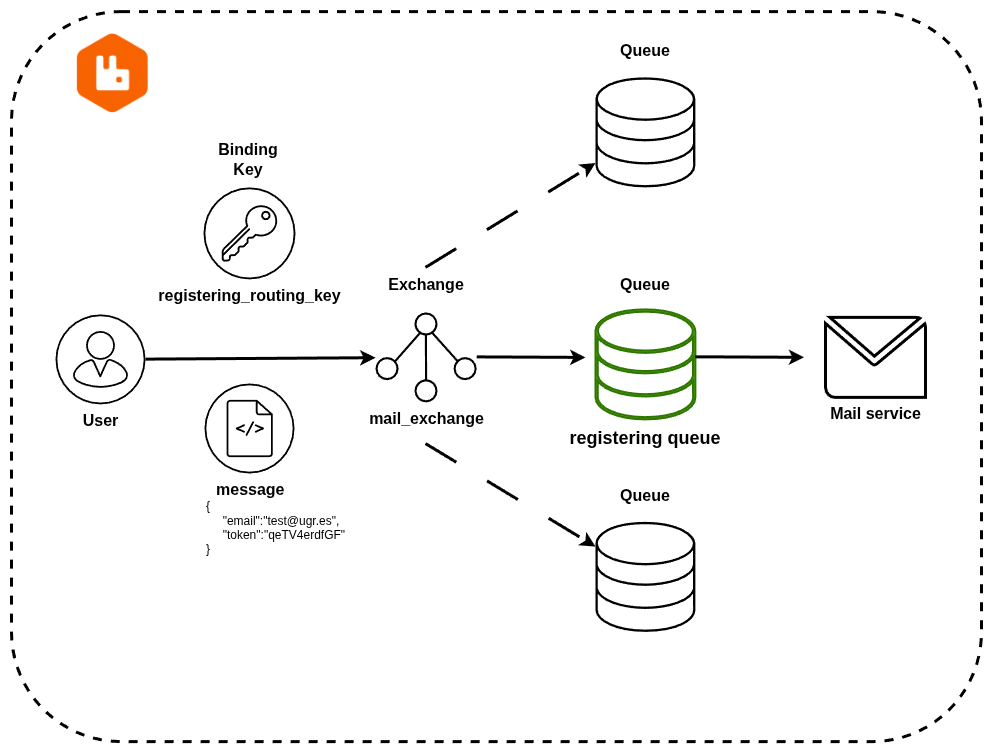
\includegraphics[width=0.8\textwidth]{figures/07_rabbit.png}
    \caption{Configuración de RabbitMQ en el servicio mail-service}
    \label{fig:rabbitmq-config}
\end{figure}

\subsubsection{Reintentos automáticos y Dead Letter Queues}

Una característica importante de la configuración es la gestión de reintentos automáticos y colas de mensajes muertos (DLQ).

Los reintentos se configuran a través de un \texttt{RetryInterceptor}:
\begin{verbatim}
.maxAttempts(3)
.backOffOptions(1000, 2.0, 50000)
\end{verbatim}
Esto indica que, si el procesamiento de un mensaje falla, se reintentará hasta tres veces, con un intervalo inicial de 1 segundo y un multiplicador exponencial. Si después de los reintentos no se logra procesar el mensaje, este se considera fallido.

En lugar de eliminar estos mensajes fallidos, se redirigen a una \textbf{Dead Letter Queue}, en este caso \texttt{mail\_dead\_letter\_queue}, asociada a su propio \texttt{Dead Letter Exchange} (\texttt{mail\_dead\_letter\_exchange}). Esto permite su análisis posterior, ya sea manual o mediante herramientas automáticas.

\subsubsection{Resumen funcional}

En este sistema, el \texttt{user-service} publica eventos de registro de usuarios a RabbitMQ. El \texttt{mail-service} escucha la cola correspondiente y envía los correos pertinentes. En caso de fallos temporales, se aplican políticas de reintento. Si el fallo persiste, el mensaje es redirigido a una DLQ, asegurando que ningún mensaje se pierde sin ser registrado.

Esta estrategia desacopla los servicios, mejora la resiliencia del sistema, y permite manejar errores de forma controlada sin interrumpir el flujo principal de la aplicación.

\subsection{Primer hito del backend}
El primer hito del backend se alcanza con la implementación de los servicios de autenticación y gestión de usuarios, junto con el servicio de correo electrónico. Estos servicios permiten registrar usuarios, autenticar sus credenciales y enviar correos electrónicos de confirmación. Además, se ha implementado el API Gateway para centralizar las peticiones y gestionar la seguridad mediante JWT.
\newline\newline
El siguiente paso antes de comenzar el siguiente sprint, y tras la reunión con Alberto Guillén Perales, es investigar cómo se pueden obtener los horarios de las asignaturas de la UGR.
\newline\newline
Para ello se investiga el sistema de scrapping, y se implementa un primer prototipo que permite obtener los horarios de las asignaturas de la UGR. Este prototipo se implementa en una primera aproximación del servicio \texttt{schedule-consumer-service}, que se encargará de consumir los horarios de las asignaturas y generar eventos a partir de ellos.
\newline
La tecnología seleccionada para realizar la tarea de scrapping es \textbf{Jsoup}, una biblioteca de Java que permite extraer y manipular datos de documentos HTML. Jsoup proporciona una API sencilla para navegar por el DOM, seleccionar elementos y extraer información, lo que facilita la tarea de scrapping.

\subsubsection{Scrapping con Jsoup}

El sistema realiza un proceso de extracción automatizado desde un portal académico para recopilar información sobre titulaciones, asignaturas, profesorado, grupos y horarios, utilizando técnicas de \textit{web scraping} con la biblioteca \texttt{Jsoup} y almacenamiento en base de datos mediante repositorios JPA.

La primera fase del proceso consiste en acceder al portal principal de ramas de conocimiento, desde donde se extraen los enlaces hacia las distintas titulaciones. A partir de cada enlace, se accede a la página específica de la titulación y se recogen sus datos básicos. Si la titulación no está ya registrada en la base de datos, se crea una nueva entrada con su nombre, URL y rama correspondiente.

Posteriormente, se recorre cada titulación almacenada y se accede a su página detallada para obtener dos tipos de información. Por un lado, si no se ha registrado la facultad correspondiente, se extrae de una tabla presente en el sitio web. Por otro lado, se recopilan los enlaces de todas las asignaturas que pertenecen a dicha titulación. Estas asignaturas se crean en la base de datos sólo si no existen previamente, y se asocian con la titulación correspondiente.

La última fase del proceso accede a cada una de las asignaturas almacenadas para extraer información detallada. En primer lugar, se recoge la información general de la asignatura como el curso académico, el año, el semestre, el tipo y el departamento responsable. Se aplican medidas de control como el recorte del texto del departamento si excede una longitud determinada.

Después, se identifica al profesorado vinculado a la asignatura y a sus respectivos grupos. Si el grupo ya existe, se actualiza su lista de profesores. Si no existe, se crea y se almacena junto con el nombre del profesor. Se contempla la posibilidad de que algunos grupos no aparezcan explícitamente en la web, en cuyo caso se generan automáticamente.

Finalmente, se extrae el horario de clases para cada grupo, identificando el día de la semana, aula, fechas de inicio y fin, y horas de inicio y fin. Esta información se transforma en objetos de clase que se asocian con el grupo correspondiente. Si no se detecta una clase idéntica en la base de datos, se crea una nueva entrada para ella.

Este enfoque permite consolidar una base de datos académica completa, dinámica y precisa, ideal para ser explotada por nuestro sistema.

\section{Sprint 2}

Se afina el scrapping, se crea el servicio schedule-consumer-service, y se crea la lógica de suscripciones a grupos, y demás tareas relacionadas. Además se puede extraer el ".ics"
de los horarios personalizados, para ello se implementa el academic-subscription-service.

Se crea además el servidor de descubrimiento de servicios con eureka, y así se investiga como mejorar el rendimiento con balanceo de carga y varias instancias.

\section{Sprint 3}

Fin del backend generando eventos a nivel de grupo y a nivel de facultad. Extracción del ics con clases oficiales, clases extra y eventos de facultad. Sincronización con Google calendar.
Alertas cuando se crean eventos a nivel de grupo (clases extra).
Se crean pruebas unitarias y se realizan pruebas de carga en el servidor de despliegue.
Se dockeriza el sistema y se implementa en un servidor de producción.

\section{Sprint 4}

Comienzo del frontend, se implementan las mismas historias de usuario que en el backend.
Refinamiento del backend, añadidos para complementar el frontend. Se añade la posibilidad de suscripcion a asignaturas por nombre de profesor.

\section{Sprint 5}

Se acaba el frontend. Se termina la documentación del proyecto. Se añade recuperación de contraseña. Se despliega y se hacen las pruebas de carga.
Se comienza la presentación del TFG.


